\setAuthor{Hans Daniel Kaimre}
\setRound{lahtine}
\setYear{2020}
\setNumber{G 3}
\setDifficulty{3}
\setTopic{TODO}

\prob{U-klaas}
\begin{wrapfigure}[6]{r}{0.25\linewidth}
		\vspace{-10pt}
		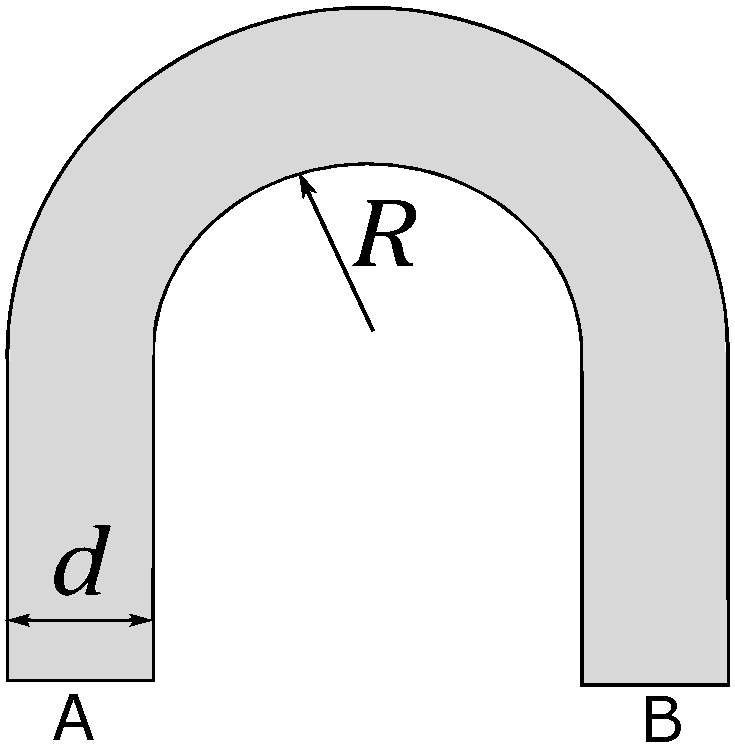
\includegraphics[width=\linewidth]{2020-lahg-03-yl.pdf}
	\end{wrapfigure}
	U-kujulise klaastüki (vt joonist) ristlõige on ristkülik. Tahule A langeb selle pinnaga risti paralleelne valgusvihk.  Millist tingimust peaks rahuldama sisemise külje kõverusraadius $R$, et kogu pealelangev valgus väljuks tahust B? Struktuuri laius $d=\SI{3}{\cm}$, klaasi murdumisnäitaja $n=\num{1.5}$ ning tahud A ja B on kaetud peegeldumisvastase kilega.
	
	
	
\hint

\solu
Esmalt teeme selgeks, milline peaks olema kõverusraadius, et esimese peegelduse jaoks oleks kogu valgusvihu ulatuses langemisnurk suurem kui kriitiline nurk. On ilmne, et kõige väiksem on langemisnurk valgusvihu kõige sisemise (joonisel parempoolse) kiire jaoks. Joonistame kiire käigu kriitilise nurga korral.

\begin{center}
	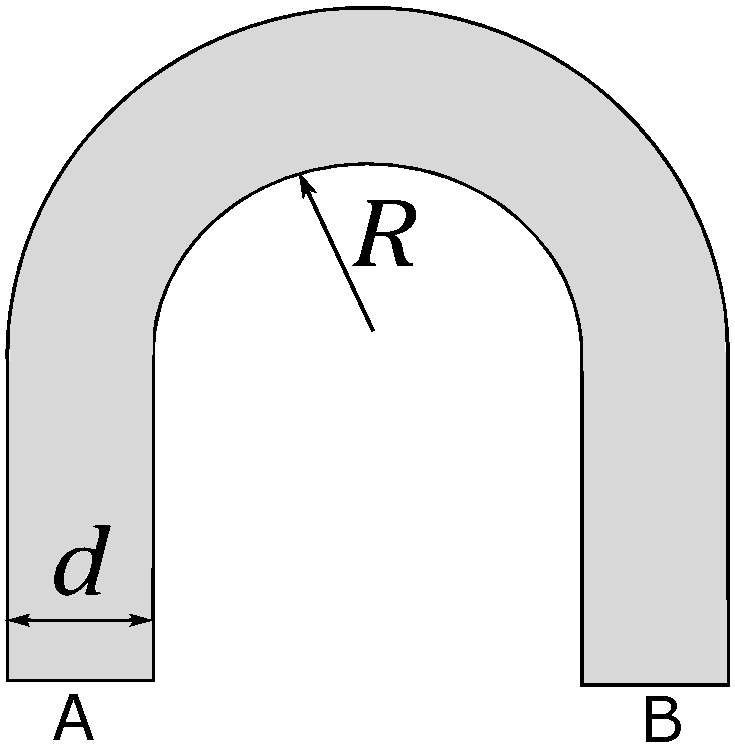
\includegraphics[width=0.6\textwidth]{2020-lahg-03-yl.pdf} 
\end{center}

Snelli seadusest täieliku sisepeegeldumise jaoks
$\sin\theta_c = {1}/{n}$, jooniselt saame, et $\sin\theta_c=R/(R+d)$. Seega
$$\frac{1}{n}=\frac{R}{R+d}\Rightarrow R = \frac{\SI{3}{\cm}}{1.5-1}=\SI{6}{cm}.$$
Paneme tähele, et peegeldunud kiir puutub sümmeetria tõttu klaasitüki sisekülge ning peegeldub välisküljelt sama nurga all kui esimene kord. Sama protsess kordub, kuni klaasi kõver osa läheb üle sirgeks. Sellisel juhul on langemisnurk suurem kui enne ning toimub kindlasti peegeldumine ja lõpuks on tagatud, et valgusvihk väljub läbi tahu B. Järelikult ongi ainsaks tingimuseks esimesest peegeldusest saadu, mis annab $R\geq\SI{6}{\cm}$.
\probend